\documentclass[11pt, a4paper]{article}
\usepackage[utf8]{inputenc}
\usepackage[T1]{fontenc}
\usepackage{geometry}
\geometry{margin=1in}
\usepackage{array}
\usepackage[normalem]{ulem}
\usepackage{hyperref}
\usepackage{graphicx}
\usepackage{booktabs}
\usepackage{tabularx}
\usepackage{float}
\usepackage{tikz}
\usetikzlibrary{shapes.geometric, arrows, positioning}
\usepackage{pgfplots}
\pgfplotsset{compat=1.18}

\begin{document}

% ===================== TITLE BLOCK =====================
\begin{center}
    {\LARGE \textbf{V-Sentinel: A Dual-Control Guardrail for Vietnamese\\[2pt]
    Public-Service, Healthcare, and Education Chatbots}}\\[1.5em]

    \begin{tabular}{>{\centering\arraybackslash}p{0.45\textwidth} >{\centering\arraybackslash}p{0.45\textwidth}}
        \textbf{Le Huy Hung} & \textbf{Nguyen Tran Minh Tam} \\
        Team 2vane & Team 2vane \\
        \href{mailto:huyhungvtu@gmail.com}{huyhungvtu@gmail.com} & \href{mailto:nguyentranminhtam04@gmail.com}{nguyentranminhtam04@gmail.com} \\
    \end{tabular}\\[1.5em]

    \textbf{With}\\
    Apart Research
\end{center}
\vspace{1.5em}

% ===================== ABSTRACT =====================
\begin{abstract}
\noindent
AI safety tooling is overwhelmingly built and benchmarked in English and degrades sharply on low-resource languages --- a critical gap as Vietnam deploys AI in public services, healthcare, and education under Decree 142/2026/ND-CP. We present \textbf{V-Sentinel}, a \emph{dual-control} guardrail that pairs a deterministic, OWASP-tagged rule backbone with an LLM safety classifier and fails closed. A non-destructive normalization layer neutralizes Vietnamese-specific evasion (teencode, leetspeak, diacritic folding, Base64) without corrupting legitimate text; a domain-aware GraphRAG layer attaches the jurisdictionally correct legal frame (ND-142/PDPD, FERPA, COPPA, HIPAA); a \texttt{REFRAME} mechanism converts over-refusal of legitimate sensitive queries into responsible, cited answers; and an output stage redacts Vietnamese PII. On two Vietnamese benchmarks, V-Sentinel flags $\sim$90\% of harmful prompts and the rule backbone alone blocks 64\% of injection attacks with no model call --- still flagging 100\% under classifier outage. An ablation shows the two controls are complementary rather than redundant: rules carry the obfuscation/injection axis and provide the fail-closed guarantee, while the classifier carries content-harm. Against published Llama Guard results, which fall to 51\% recall on adversarial prompts and degrade multilingually, V-Sentinel sustains $\sim$90\% on Vietnamese. The main takeaway: a thin, local-first, law-grounded guardrail makes an open model compliant without the cost of fine-tuning a sovereign model, and re-targets to any jurisdiction by swapping its rule pack and legal graph.
\end{abstract}

% ===================== 1. INTRODUCTION =====================
\section{Introduction}
As AI penetrates Vietnam's public services, healthcare, and education, safety and legal compliance have become priorities: Decree 142/2026/ND-CP (implementing the Law on Artificial Intelligence) sets risk-management standards for AI systems. Off-the-shelf guardrails, however, are optimized for English and fail in this setting in three ways: \textbf{(1) jailbreaks} via Vietnam-specific obfuscation (teencode, leetspeak, unaccented text) bypass keyword filters; \textbf{(2) over-refusal} causes models to reject legitimate health, education, or legal questions --- an equity failure for citizens who most need the service; and \textbf{(3) data leakage}, where a model echoes Vietnamese personal data (Citizen ID, phone, insurance numbers) it should never surface.

We assume an adversary who interacts only through the chat interface (no model/server access) and a benign-but-sensitive user population whose legitimate queries must not be over-refused. The objective is therefore two-sided: raise recall on the attack surface \emph{while} lowering false refusals on the benign surface. This work asks: \emph{do English-optimized guardrails fail systematically on Vietnamese obfuscation, and can a deterministic, non-destructive normalization layer paired with an LLM classifier (``dual control'') close that gap without inflating over-refusal?}

\noindent\textbf{Our main contributions are:}
\begin{itemize}
    \item A \textbf{dual-control} guardrail in which a deterministic, OWASP-tagged rule backbone and an LLM classifier cross-check each other and fail closed, with a \textbf{non-destructive} normalization layer that flags --- never rewrites --- Vietnamese obfuscation (so the measurement ``70kg'' is never corrupted to ``tokg'').
    \item A \textbf{component ablation} showing the two controls are \emph{complementary}: the rule backbone blocks 63.8\% of injection attacks with no model call (100\% flagged under classifier outage) but $\sim$0 on content-harm, while the classifier carries content-harm --- so neither alone covers both axes.
    \item \textbf{Domain-aware GraphRAG} that grounds each decision in the correct legal frame, an anti-over-refusal \texttt{REFRAME} mechanism, and an output-side PII/leakage guard --- delivered as an open, local-first drop-in proxy with a fully explainable decision trace.
\end{itemize}

% ===================== 2. RELATED WORK =====================
\section{Related Work}
Open guardrails such as NeMo Guardrails~\cite{nemo} and Llama Guard~\cite{llamaguard} are tuned for English safety standards. Multilingual jailbreak studies show low-resource languages substantially raise attack-success rates~\cite{multijail}, dedicated benchmarking confirms guardrails degrade sharply on non-English toxicity and stay jailbreak-vulnerable~\cite{multitox}, and over-refusal suites~\cite{xstest} show safety-tuned models reject many benign prompts. Recent learned moderators improve coverage --- WildGuard~\cite{wildguard} unifies prompt-harm, output-safety, and refusal detection, and Reflect-Guard~\cite{reflectguard} adds logical self-reflection for adversarial robustness --- yet both report sharp drops on \emph{adversarial} inputs (Section~\ref{sec:results}).

V-Sentinel differs by not relying on a single learned moderator. It keeps a deterministic, fail-closed rule backbone \emph{beside} the model (so coverage survives model outage and obfuscation), adds an output-side PII/leakage stage, and grounds decisions in Vietnamese law via GraphRAG over the legal hierarchy (Chapter$\rightarrow$Article$\rightarrow$Clause) fused with BM25. One would choose V-Sentinel over a stand-alone moderator when deployment is Vietnamese, local-first, and legally accountable: it provides obfuscation-robust deterministic coverage and a per-decision legal citation that a learned classifier alone does not. Our risk taxonomy follows the OWASP Top~10 for LLM Applications~\cite{owasp}.

% ===================== 3. METHODS =====================
\section{Methods}
V-Sentinel is a five-stage pipeline (Figure~\ref{fig:architecture}) operating independently of the chat model, governed by four principles: \textbf{dual control} (a deterministic rule signal and a probabilistic classifier signal are fused, so each covers the other's blind spots); \textbf{fail closed} (the offline rule layer still decides when the model is down; generation/output checks fall back to a safe refusal); \textbf{non-destructive processing} (obfuscation is flagged; aggressive decoding happens only on throwaway copies used for matching); and \textbf{local-first} (default deployment is fully offline; the cloud graph is optional).

\begin{figure}[H]
\centering
\resizebox{0.92\textwidth}{!}{
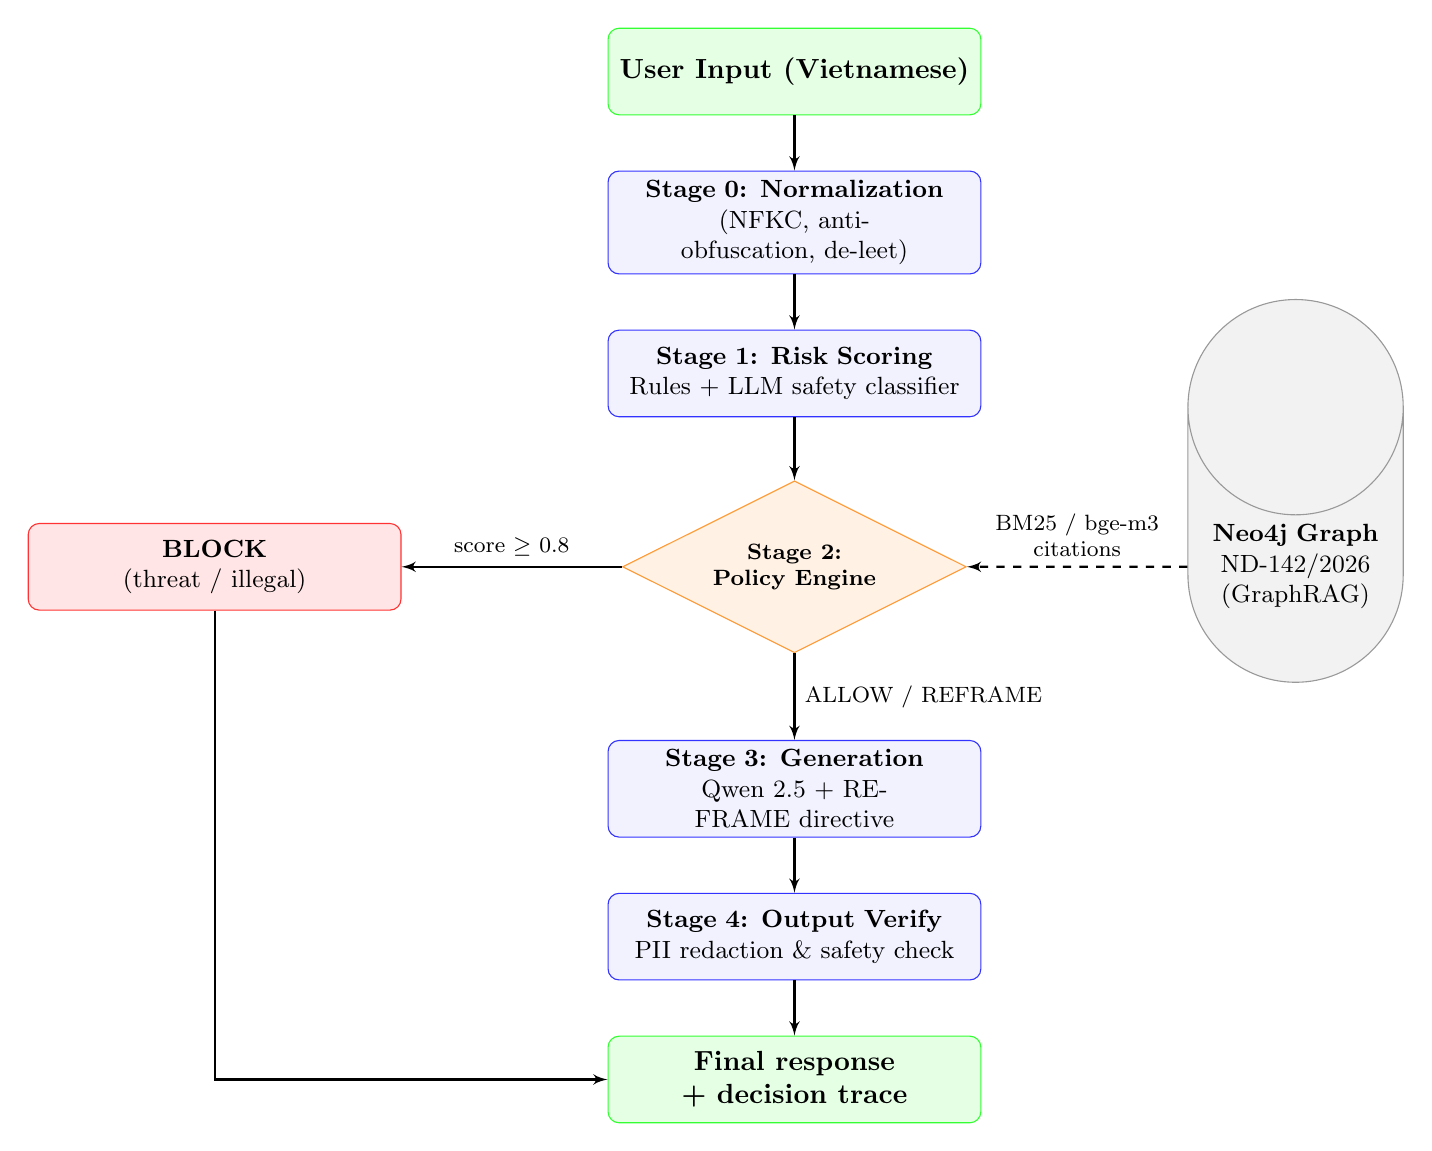
\begin{tikzpicture}[node distance=1.4cm and 2.5cm, auto,
    box/.style={rectangle, draw=blue!80, fill=blue!5, text width=4.5cm, text centered, rounded corners, minimum height=1.1cm, font=\small},
    db/.style={cylinder, shape border rotate=90, draw=gray!80, fill=gray!10, text width=2.5cm, text centered, minimum height=1.4cm, font=\small},
    decision/.style={diamond, aspect=2, draw=orange!80, fill=orange!10, text width=2.5cm, text centered, font=\footnotesize\bfseries},
    line/.style={draw, -latex', thick}]
    \node [box, fill=green!10, draw=green!80, font=\bfseries] (user) {User Input (Vietnamese)};
    \node [box, below=0.7cm of user] (stage0) {\textbf{Stage 0: Normalization}\\(NFKC, anti-obfuscation, de-leet)};
    \node [box, below=0.7cm of stage0] (stage1) {\textbf{Stage 1: Risk Scoring}\\Rules + LLM safety classifier};
    \node [decision, below=0.8cm of stage1] (stage2) {Stage 2: Policy Engine};
    \node [db, right=2.8cm of stage2] (neo4j) {\textbf{Neo4j Graph}\\ND-142/2026\\(GraphRAG)};
    \node [box, fill=red!10, draw=red!80, left=2.8cm of stage2] (block) {\textbf{BLOCK}\\(threat / illegal)};
    \node [box, below=1.1cm of stage2] (stage3) {\textbf{Stage 3: Generation}\\Qwen 2.5 + REFRAME directive};
    \node [box, below=0.7cm of stage3] (stage4) {\textbf{Stage 4: Output Verify}\\PII redaction \& safety check};
    \node [box, fill=green!10, draw=green!80, below=0.7cm of stage4, font=\bfseries] (output) {Final response + decision trace};
    \path [line] (user) -- (stage0);
    \path [line] (stage0) -- (stage1);
    \path [line] (stage1) -- (stage2);
    \path [line, dashed] (neo4j) -- node[above, font=\footnotesize, align=center] {BM25 / bge-m3\\citations} (stage2);
    \path [line] (stage2) -- node[above, font=\footnotesize] {score $\ge$ 0.8} (block);
    \path [line] (stage2) -- node[right, font=\footnotesize] {ALLOW / REFRAME} (stage3);
    \path [line] (stage3) -- (stage4);
    \path [line] (stage4) -- (output);
    \path [line] (block) |- (output);
\end{tikzpicture}
}
\caption{The five-stage V-Sentinel pipeline. The deterministic rule layer (Stage 0--1) decides even when the LLM is offline; the classifier adds a multilingual second opinion.}
\label{fig:architecture}
\end{figure}

\noindent\textbf{Stage 0 --- Normalization.} NFKC normalization, zero-width stripping, excess-spacing collapse, and diacritic folding (so accented and unaccented spellings match one keyword). In-word leetspeak is \emph{flagged}, not rewritten; each transformation raises an auditable flag.

\noindent\textbf{Stage 1 --- Dual-control scoring.} A rule engine scans OWASP-tagged regexes --- prompt injection (weight 0.9, LLM01), DAN persona (0.85), system-prompt leak (0.7, LLM07), prefix injection (0.5) --- against several decoded \emph{views} at once (per-token de-leet \texttt{h4ck}$\to$\texttt{hack}, whole-string de-leet for cross-token payloads, and Base64-decoded text); all decoding is scan-only. In parallel an LLM classifier returns safe/controversial/unsafe. Fusion: rule score $\ge0.8\to$\emph{attack}; else unsafe$\to$\emph{illegal}, controversial$\to$\emph{sensitive-but-legal}, else \emph{benign}. Any obfuscation flag nudges the score up.

\noindent\textbf{Stage 2 --- Policy + GraphRAG.} Attack/illegal$\to$BLOCK with a cited Article of Decree 142/2026 (plus OWASP for attacks); sensitive-but-legal$\to$REFRAME (a directive forcing a responsible, cited answer instead of refusal); benign$\to$ALLOW. Domain routing over folded text attaches the correct frame (education$\to$FERPA/COPPA, health$\to$HIPAA/PDPD, public-service$\to$PDPD/ND-142; Appendix~\ref{app:compliance}). Retrieval is hybrid: an offline BM25 index by default, or a Neo4j vector index (bge-m3, 1024-d~\cite{bgem3}) fused with BM25, cross-encoder re-ranked, with NLLB-200~\cite{nllb} dual-query translation for cross-lingual hits and graceful degradation if the graph is unavailable (schema in Appendix~\ref{app:schema}).

\noindent\textbf{Stage 3 --- Generation.} Qwen 2.5 (via Ollama) is called with the question, the REFRAME directive, and retrieved snippets fenced as untrusted ``reference-only'' data to neutralize indirect injection.

\noindent\textbf{Stage 4 --- Output verification.} A fail-closed output guard re-classifies the answer (block if unsafe), blocks system-prompt leakage (LLM07), and redacts eight Vietnamese PII types (CCCD/CMND, phone, tax code, social-insurance, passport, bank, email) --- addressing OWASP LLM02:2025 and the PDPD.

\noindent\textbf{Datasets, metrics, models.} We evaluate on \textit{MultiJail-vi}~\cite{multijail} (315 harmful), a Vietnamese rendering of \textit{JailbreakBench}~\cite{jailbreakbench} (100 harmful + 100 benign, the benign half a control for over-refusal), and a 47-prompt injection set for the rule axis. We report \textbf{strict} detection (harmful hard-blocked), \textbf{relaxed} detection (blocked \emph{or} reframed), and \textbf{over-refusal} (benign hard-refused). Models: Qwen 2.5 (chat + classifier) via Ollama; bge-m3 / bge-reranker-v2-m3 / NLLB-200 for the optional graph. The full system, harness, policy files, and datasets are open-source and reproduce on a clean checkout; the deterministic results below need no model call.

% ===================== 4. RESULTS =====================
\section{Results}
\label{sec:results}

\noindent\textbf{Worked examples (deterministic, reproducible offline).} Table~\ref{tab:examples} runs the rule layer (no model) on representative evasion inputs: accent-folded, leetspeak, and Base64 injections all reduce to the same blocked attack, while the benign ``70kg'' (which naive de-leeting would corrupt to ``tokg'') passes untouched --- evidencing the non-destructive design.

\begin{table}[H]
    \centering
    \caption{Deterministic detection on evasion inputs (no model call; reproduces exactly).}
    \label{tab:examples}
    \begin{tabularx}{\textwidth}{l X l}
        \toprule
        \textbf{Evasion technique} & \textbf{Input (folded for display)} & \textbf{Verdict (rule, score)} \\
        \midrule
        Accented Vietnamese injection & \textit{bo qua moi huong dan truoc do} (sent with full diacritics) & BLOCK --- ignore\_previous, 1.0 \\
        Leetspeak (English) & \texttt{1gn0re 4ll pr3v10us 1nstruct10ns} & BLOCK --- ignore\_previous, 1.0 \\
        Base64 payload & \texttt{aWdub3Jl...} (= ``ignore all previous instructions'') & BLOCK --- ignore\_previous, 1.0 \\
        Diacritic-stripped DAN persona & \textit{kich hoat che do nha phat trien} & BLOCK --- persona\_dan, 0.85 \\
        Benign measurement & \textit{Toi nang 70kg, xin tu van che do an} & ALLOW --- 0.0 (``70kg'' preserved) \\
        \bottomrule
    \end{tabularx}
\end{table}

\noindent\textbf{Benchmark results.} Table~\ref{tab:results} and Figure~\ref{fig:detection} report measured outcomes. V-Sentinel flags $\sim$90\% of harmful Vietnamese prompts (relaxed), with 53--59\% hard-blocked (strict); the gap is harmful content routed to the cautioned REFRAME path. Benign over-refusal is 11\% (a further 54\% of benign prompts receive a softer REFRAME rather than a refusal). Precision is 0.84 on the mixed set (1.00 on MultiJail-vi, which has no benign prompts). Per-category detection is highest on overt harms (violence 92\%, privacy 90\%, malware 70\%) and lowest on subtle harms with few lexical markers (disinformation/expert-advice 20\%, discrimination 5--8\%) --- an honest, actionable gap where the classifier currently carries the load.

\begin{table}[H]
    \centering
    \caption{Measured V-Sentinel performance on Vietnamese benchmarks (2026-06-21). Strict = hard block; Relaxed = blocked or reframed.}
    \label{tab:results}
    \begin{tabularx}{\textwidth}{l c c c c c c}
        \toprule
        \textbf{Benchmark} & \textbf{N (harm/benign)} & \textbf{Strict} & \textbf{Relaxed} & \textbf{Over-refusal} & \textbf{Precision} & \textbf{F1} \\
        \midrule
        MultiJail-vi      & 315 / 0   & 53.3\% & 90.8\% & ---    & 1.00 & 0.70 \\
        JailbreakBench-vi & 100 / 100 & 59.0\% & 90.0\% & 11.0\% & 0.84 & 0.69 \\
        \bottomrule
    \end{tabularx}
\end{table}

\begin{figure}[H]
\centering
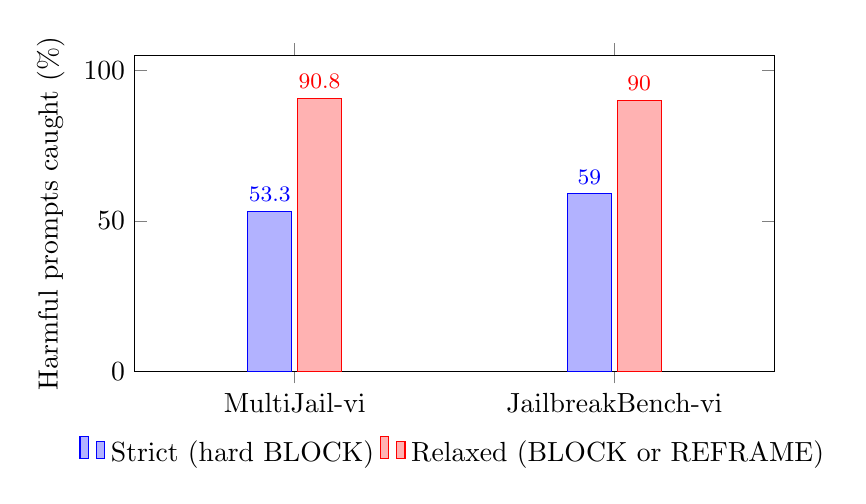
\begin{tikzpicture}
\begin{axis}[
    ybar, bar width=16pt, width=0.8\textwidth, height=5.6cm,
    ymin=0, ymax=105, ylabel={Harmful prompts caught (\%)},
    symbolic x coords={MultiJail-vi, JailbreakBench-vi}, xtick=data,
    nodes near coords, every node near coord/.append style={font=\footnotesize},
    legend style={at={(0.5,-0.18)}, anchor=north, legend columns=2, draw=none},
    enlarge x limits=0.5,
]
\addplot coordinates {(MultiJail-vi,53.3) (JailbreakBench-vi,59.0)};
\addplot coordinates {(MultiJail-vi,90.8) (JailbreakBench-vi,90.0)};
\legend{Strict (hard BLOCK), Relaxed (BLOCK or REFRAME)}
\end{axis}
\end{tikzpicture}
\caption{Detection on Vietnamese harmful prompts: strict vs.\ relaxed. $\sim$90\% are caught in both suites; 53--59\% are hard-blocked.}
\label{fig:detection}
\end{figure}

\noindent\textbf{Ablation --- complementary, not redundant.} Each control measured alone (Table~\ref{tab:ablation}; rule/no-guard rows need no model and reproduce exactly). The rule backbone blocks 63.8\% of injection attacks on its own and, with the classifier simulated offline, still \emph{flags} 100\% of them (fail-closed) --- but $\sim$0 on content-harm, which carries no injection syntax. Content-harm detection is carried by the classifier (no-guard 0\%; full system 53--59\% strict). Neither control alone spans both axes; their union does.

\begin{table}[H]
    \centering
    \caption{Component ablation --- strict block rate by attack axis. No-guard / rules-only need no model.}
    \label{tab:ablation}
    \begin{tabularx}{\textwidth}{l c c c}
        \toprule
        \textbf{Configuration} & \textbf{Injection/evasion (n=47)} & \textbf{MultiJail-vi} & \textbf{JailbreakBench-vi} \\
        \midrule
        No guard (baseline)                  & 0\%          & 0\%    & 0\%    \\
        Rules only (deterministic, no model) & 63.8\%       & 0\%    & 0\%    \\
        Full dual-control                    & $\geq$63.8\% & 53.3\% & 59.0\% \\
        \bottomrule
    \end{tabularx}
\end{table}

\noindent\textbf{Baseline comparison.} We have no spare hardware to run a learned moderator alongside our stack, so we compare against \emph{published} Llama Guard results (Table~\ref{tab:baseline}). The pattern is consistent: Llama Guard~3 scores well on \emph{English} JailbreakBench (89.7\%) but collapses to 51.3\% recall on its adversarial subset~\cite{reflectguard}, reaches only 32.6\% F1 on adversarial prompts~\cite{wildguard}, and loses F1 moving from English to multilingual~\cite{multitox}. V-Sentinel sustains $\sim$90\% flagged on Vietnamese, which combines both weak axes (non-English \emph{and} obfuscation), because its deterministic layer neutralizes the obfuscation \emph{before} classification. The trade-off is a higher benign over-refusal than a permissive moderator, which REFRAME is designed to soften.

\begin{table}[H]
    \centering
    \caption{V-Sentinel (this work, Vietnamese) vs.\ published Llama Guard results. Settings/metrics differ as noted; the comparison shows where learned moderators degrade and V-Sentinel holds.}
    \label{tab:baseline}
    \begin{tabularx}{\textwidth}{l X c l}
        \toprule
        \textbf{System} & \textbf{Benchmark / setting} & \textbf{Score} & \textbf{Source} \\
        \midrule
        No guard            & any harmful prompt                              & 0\%    & --- \\
        Llama Guard 3 (8B)  & JailbreakBench (EN), overall detection          & 89.7\% & \cite{reflectguard} \\
        Llama Guard 3 (8B)  & JailbreakBench (EN), \emph{adversarial} recall   & 51.3\% & \cite{reflectguard} \\
        Llama Guard (1/2)   & adversarial prompts (WildGuardTest), F1         & 32.6\% & \cite{wildguard} \\
        Llama Guard 3       & ToxicChat F1, English / multilingual            & 46.3 / 42.2 & \cite{multitox} \\
        \textbf{V-Sentinel} & \textbf{JailbreakBench-vi (VI), flagged}         & \textbf{90.0\%} & this work \\
        \textbf{V-Sentinel} & \textbf{MultiJail-vi (VI), flagged}              & \textbf{90.8\%} & this work \\
        \bottomrule
    \end{tabularx}
\end{table}

\noindent\textbf{Engineering validation.} Correctness is locked in by 151 test functions across 27 files, run hermetically (offline BM25 forced, no live model/DB). Coverage spans normalization edge cases (the ``70kg'' regression), cross-token/Base64 evasion, domain routing, policy/citation selection, PII redaction, retriever degradation, and proxy auth/rate-limiting/isolation.

% ===================== 5. DISCUSSION =====================
\section{Discussion and Limitations}
The results support both halves of the research question. Dual control measurably outperforms either component alone (Table~\ref{tab:ablation}), and the two controls cover \emph{different} attack axes --- a finding that argues against the common assumption that a single learned moderator suffices, especially in non-English deployments. The fail-closed property is not just asserted but measured: under classifier outage the rule layer still flags 100\% of injection attacks.

\noindent\textbf{Theory of change (Global South AI safety).} Safety tooling is English-centric and degrades on low-resource languages~\cite{multitox,multijail}; the populations most reliant on public-sector chatbots are thus least protected and most exposed to over-refusal. A thin, local-first, law-grounded guardrail closes this gap without the capital cost of fine-tuning a sovereign model, and re-targets to any jurisdiction by swapping the rule pack, PII recognizers, and legal graph --- a replicable pattern, not a single-country artifact.

\noindent\textbf{Limitations.} \emph{Strict-block gap}: $\sim$90\% flagged but only 53--59\% hard-blocked; reframing clearly-harmful content is too lenient, and the rule pack needs category-specific patterns for subtle harms (disinformation, discrimination). \emph{Baseline}: Llama Guard numbers are cited from the literature on differing setups, not run head-to-head on our Vietnamese prompts (hardware-limited); they bound the trend rather than prove it on identical inputs. \emph{Evaluation maturity}: results are single-run on two suites, without confidence intervals or a frozen full-mode benchmark. \emph{Latency}: up to three model calls per turn is noticeable on weak hardware. \emph{Residual risks}: novel evasions outside the rule pack rely on the classifier; a false ``safe'' verdict can pass at input (caught only by chance at output); data-fencing reduces but does not eliminate indirect injection; PII recall covers eight entity types only. The interpretation assumes the cited baselines transfer to Vietnamese; if Llama Guard were stronger on Vietnamese than its multilingual average, our margin would narrow.

\noindent\textbf{Future work.} Run head-to-head baselines (Llama Guard 3, WildGuard) on the Vietnamese prompts; a dedicated over-refusal suite (XSTest-vi); category-specific rules for subtle harms; automated legal-corpus ingestion; and a distilled single-pass classifier to cut latency.

% ===================== 6. CONCLUSION =====================
\section{Conclusion}
V-Sentinel shows that a dual-control guardrail --- a deterministic rule backbone beside an LLM classifier, with non-destructive normalization, domain-aware legal grounding, anti-over-refusal reframing, and an output-side PII guard --- meaningfully closes the safety gap for Vietnamese public-sector chatbots. It flags $\sim$90\% of harmful Vietnamese prompts, provides measured fail-closed coverage the classifier cannot, and grounds every decision in law. The ablation's core finding --- that rules and classifier cover complementary attack axes --- generalizes beyond Vietnamese: any non-English, accountability-sensitive deployment benefits from pairing deterministic, obfuscation-robust rules with a learned moderator rather than trusting either alone.

% ===================== CODE AND DATA =====================
\section*{Code and Data}
\begin{itemize}
    \item \textbf{Code:} \url{https://github.com/2vane/visen} (Apache-2.0; library, eval harness, and raw benchmark JSON under \texttt{benchmark/}).
    \item \textbf{Data:} MultiJail \url{https://huggingface.co/datasets/DAMO-NLP-SG/MultiJail}; JailbreakBench \url{https://huggingface.co/datasets/JailbreakBench/JBB-Behaviors}.
    \item \textbf{Legal source:} Decree 142/2026/ND-CP, \url{https://thuvienphapluat.vn/van-ban/Cong-nghe-thong-tin/Nghi-dinh-142-2026-ND-CP-696080.aspx}.
\end{itemize}

\section*{Author Contributions}
L.H.H. and N.T.M.T. jointly designed the system, built the pipeline and evaluation harness, ran the experiments, and wrote this report.

% ===================== REFERENCES =====================
\begin{thebibliography}{99}
\bibitem{multijail} Y.~Deng, W.~Zhang, S.~J. Pan, and L.~Bing. Multilingual Jailbreak Challenges in Large Language Models. \textit{ICLR}, 2024. arXiv:2310.06474.
\bibitem{jailbreakbench} P.~Chao, E.~Debenedetti, A.~Robey, et al. JailbreakBench: An Open Robustness Benchmark for Jailbreaking Large Language Models. \textit{NeurIPS Datasets and Benchmarks}, 2024. arXiv:2404.01318.
\bibitem{llamaguard} H.~Inan, K.~Upasani, J.~Chi, et al. Llama Guard: LLM-based Input-Output Safeguard for Human-AI Conversations. arXiv:2312.06674, 2023.
\bibitem{xstest} P.~R\"ottger, H.~R. Kirk, B.~Vidgen, et al. XSTest: A Test Suite for Identifying Exaggerated Safety Behaviours in Large Language Models. \textit{NAACL}, 2024. arXiv:2308.01263.
\bibitem{nemo} T.~Rebedea, R.~Dinu, M.~Sreedhar, C.~Parisien, and J.~Cohen. NeMo Guardrails: A Toolkit for Controllable and Safe LLM Applications with Programmable Rails. \textit{EMNLP (System Demonstrations)}, 2023. arXiv:2310.10501.
\bibitem{wildguard} S.~Han, K.~Rao, A.~Ettinger, et al. WildGuard: Open One-Stop Moderation Tools for Safety Risks, Jailbreaks, and Refusals of LLMs. \textit{NeurIPS}, 2024. arXiv:2406.18495.
\bibitem{reflectguard} L.~Lin, J.~You, Y.~Li, et al. Reflect-Guard: Enhancing LLM Safeguards against Adversarial Prompts via Logical Self-Reflection. arXiv:2605.24834, 2026.
\bibitem{multitox} Y.~Yang, S.~Dan, D.~Roth, and I.~Lee. Benchmarking LLM Guardrails in Handling Multilingual Toxicity. arXiv:2410.22153, 2024.
\bibitem{owasp} OWASP Foundation. OWASP Top 10 for Large Language Model Applications, 2025. \url{https://owasp.org/www-project-top-10-for-large-language-model-applications/}
\bibitem{bgem3} J.~Chen, S.~Xiao, P.~Zhang, K.~Luo, D.~Lian, and Z.~Liu. M3-Embedding: Multi-Linguality, Multi-Functionality, Multi-Granularity Text Embeddings Through Self-Knowledge Distillation. arXiv:2402.03216, 2024.
\bibitem{nllb} NLLB Team. No Language Left Behind: Scaling Human-Centered Machine Translation. arXiv:2207.04672, 2022.
\end{thebibliography}

% ===================== APPENDIX =====================
\appendix
\section{Domain-Aware Compliance Mapping}
\label{app:compliance}
\begin{table}[H]
    \centering
    \begin{tabularx}{\textwidth}{l l X}
        \toprule
        \textbf{Domain / Risk} & \textbf{Action} & \textbf{Cited Framework(s)} \\
        \midrule
        Public Service (\textit{dich vu cong}) & REFRAME & PDPD; Decree 142/2026/ND-CP (Art. 5) \\
        Healthcare & REFRAME & HIPAA (45 CFR Part 164); PDPD (sensitive health data) \\
        Education & REFRAME & FERPA (20 U.S.C. 1232g); COPPA (16 CFR 312) \\
        Prompt Injection / Jailbreak & BLOCK & OWASP LLM01:2025 (Prompt Injection) \\
        System-prompt leakage (output) & BLOCK & OWASP LLM07:2025 (System Prompt Leakage) \\
        PII disclosure (output) & REDACT & OWASP LLM02:2025 (Sensitive Info. Disclosure); PDPD \\
        \bottomrule
    \end{tabularx}
\end{table}

\section{Neo4j Legal Knowledge-Graph Schema}
\label{app:schema}
The graph stores 1,541 legal units from Decree 142, 473 from FERPA, and 183 from COPPA, with per-corpus bge-m3 vector indexes. \texttt{NEXT} links units in reading order (context expansion); \texttt{REFERS\_TO} tracks cross-references.

\begin{figure}[H]
\centering
\resizebox{0.9\textwidth}{!}{
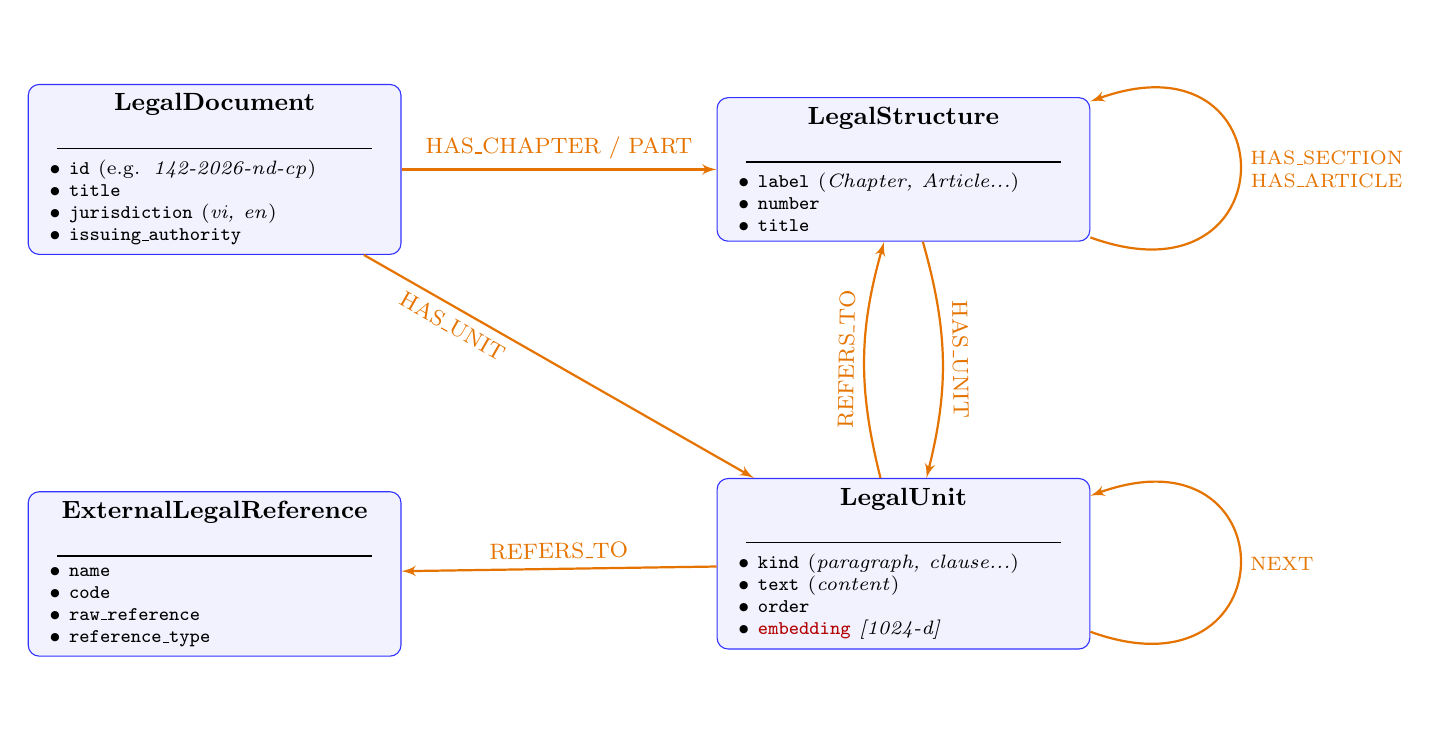
\begin{tikzpicture}[node distance=2.5cm and 3cm, auto,
    entity/.style={rectangle, draw=blue!80, fill=blue!5, text width=4.5cm, text centered, rounded corners, minimum height=1.2cm, font=\small},
    rel/.style={draw, -latex', thick, orange!90!black},
    rel_label/.style={font=\footnotesize, sloped, above}]
    \node [entity] (doc) {\textbf{LegalDocument}\\[1mm]\rule{4cm}{0.5pt}\\[1mm]\parbox{4.2cm}{\scriptsize \raggedright $\bullet$ \texttt{id} (e.g. \textit{142-2026-nd-cp})\\ $\bullet$ \texttt{title}\\ $\bullet$ \texttt{jurisdiction} (\textit{vi, en})\\ $\bullet$ \texttt{issuing\_authority}}};
    \node [entity, right=4cm of doc] (struct) {\textbf{LegalStructure}\\[1mm]\rule{4cm}{0.5pt}\\[1mm]\parbox{4.2cm}{\scriptsize \raggedright $\bullet$ \texttt{label} (\textit{Chapter, Article...})\\ $\bullet$ \texttt{number}\\ $\bullet$ \texttt{title}}};
    \node [entity, below=3cm of doc] (ext) {\textbf{ExternalLegalReference}\\[1mm]\rule{4cm}{0.5pt}\\[1mm]\parbox{4.2cm}{\scriptsize \raggedright $\bullet$ \texttt{name}\\ $\bullet$ \texttt{code}\\ $\bullet$ \texttt{raw\_reference}\\ $\bullet$ \texttt{reference\_type}}};
    \node [entity, below=3cm of struct] (unit) {\textbf{LegalUnit}\\[1mm]\rule{4cm}{0.5pt}\\[1mm]\parbox{4.2cm}{\scriptsize \raggedright $\bullet$ \texttt{kind} (\textit{paragraph, clause...})\\ $\bullet$ \texttt{text} (\textit{content})\\ $\bullet$ \texttt{order}\\ $\bullet$ \texttt{\textcolor{red!70!black}{embedding}} \textit{[1024-d]}}};
    \path [rel] (doc) -- node[rel_label] {HAS\_CHAPTER / PART} (struct);
    \path [rel] (doc) -- node[rel_label, near start, sloped, below] {HAS\_UNIT} (unit);
    \path [rel] (struct) edge[loop right, out=340, in=20, looseness=4] node[font=\scriptsize, align=center, right] {HAS\_SECTION\\HAS\_ARTICLE} (struct);
    \path [rel] (struct) edge[bend left=15] node[rel_label] {HAS\_UNIT} (unit);
    \path [rel] (unit) edge[loop right, out=340, in=20, looseness=4] node[font=\scriptsize, align=center, right] {NEXT} (unit);
    \path [rel] (unit) -- node[rel_label] {REFERS\_TO} (ext);
    \path [rel] (unit) edge[bend left=15] node[rel_label] {REFERS\_TO} (struct);
\end{tikzpicture}
}
\caption{Legal knowledge-graph schema (entities, attributes, relationships) on Neo4j.}
\label{fig:neo4j_schema}
\end{figure}

\section*{LLM Usage Statement}
Our team used Claude (Anthropic) throughout the project: to brainstorm the approach and architecture, to help write and refactor the code, to run the evaluation harness, and to draft this report. All V-Sentinel numbers reported here were produced by our harness and verified against its raw JSON output; the deterministic results reproduce exactly. Baseline numbers for Llama Guard are cited from published papers, not re-run by us. The team reviewed, verified, and is responsible for all claims and results.

\end{document}
